\documentclass[tikz,border=4pt]{standalone}
\usepackage{tikz}
\usepackage{xcolor}
\usepackage{amsmath}

\definecolor{mleblue}{HTML}{2A78D6}
\definecolor{mleorange}{HTML}{EB6834}
\definecolor{mlegray}{HTML}{C3C2B7}
\definecolor{mleink}{HTML}{0B0B0B}
\definecolor{mlesub}{HTML}{52514E}
\definecolor{mlemut}{HTML}{898781}
\definecolor{mlegrid}{HTML}{E1E0D9}
\definecolor{mlesurf}{HTML}{FCFCFB}

\begin{document}
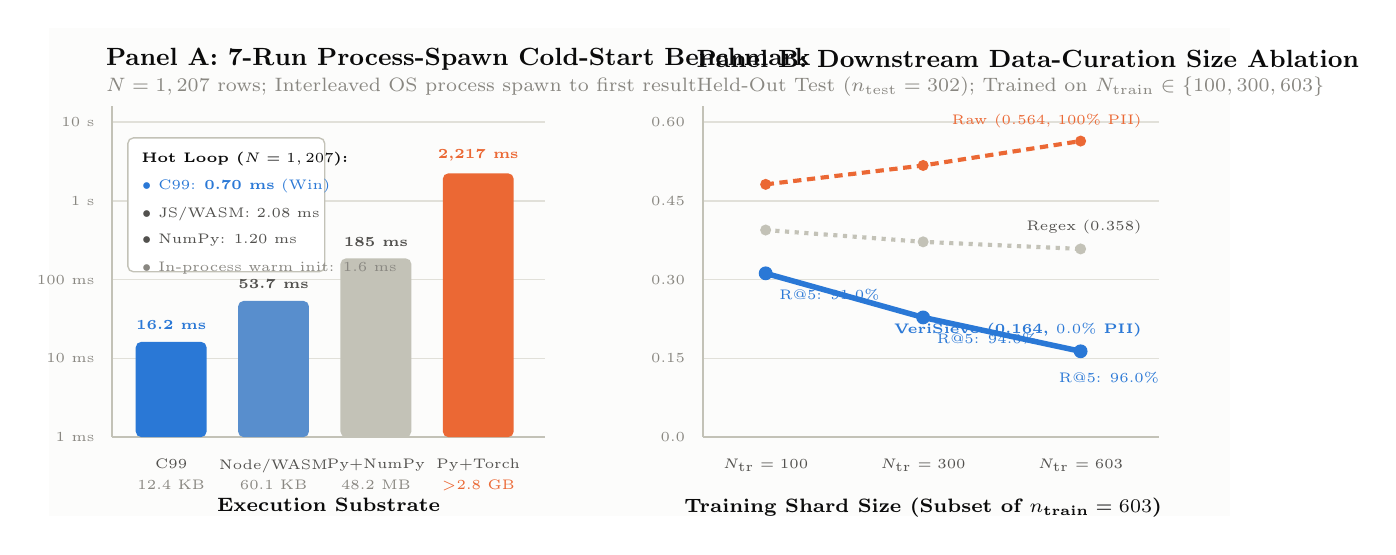
\begin{tikzpicture}[x=1cm, y=1cm, font=\sffamily]
  % Background surface
  \fill[mlesurf] (-0.8, -1.0) rectangle (14.2, 5.2);

  % ================= PANEL A =================
  \begin{scope}[shift={(0,0)}]
    \node[anchor=west, text=mleink, font=\bfseries\small] at (-0.2, 4.8) {Panel A: 7-Run Process-Spawn Cold-Start Benchmark};
    \node[anchor=west, text=mlemut, font=\scriptsize] at (-0.2, 4.45) {$N=1,207$ rows; Interleaved OS process spawn to first result};

    % Grid lines (Cold Start: log-scale 1 ms to 10 s, 4.0cm = 4 decades)
    \draw[mlegrid, line width=0.5pt] (0,0) -- (5.5,0);
    \draw[mlegrid, line width=0.5pt] (0,1.0) -- (5.5,1.0);
    \draw[mlegrid, line width=0.5pt] (0,2.0) -- (5.5,2.0);
    \draw[mlegrid, line width=0.5pt] (0,3.0) -- (5.5,3.0);
    \draw[mlegrid, line width=0.5pt] (0,4.0) -- (5.5,4.0);

    % Y Axis labels (Cold Start Latency)
    \node[anchor=east, text=mlemut, font=\tiny] at (-0.1, 0) {1 ms};
    \node[anchor=east, text=mlemut, font=\tiny] at (-0.1, 1.0) {10 ms};
    \node[anchor=east, text=mlemut, font=\tiny] at (-0.1, 2.0) {100 ms};
    \node[anchor=east, text=mlemut, font=\tiny] at (-0.1, 3.0) {1 s};
    \node[anchor=east, text=mlemut, font=\tiny] at (-0.1, 4.0) {10 s};

    % Axes
    \draw[mlegray, line width=0.8pt] (0,0) -- (5.5,0);
    \draw[mlegray, line width=0.8pt] (0,0) -- (0,4.2);

    % Bar 1: Native C99 (16.2 ms => log10(16.2) = 1.21)
    \fill[mleblue, rounded corners=2pt] (0.3, 0) rectangle (1.2, 1.21);
    \node[anchor=south, text=mleblue, font=\tiny\bfseries] at (0.75, 1.24) {16.2 ms};
    \node[anchor=north, text=mlesub, font=\tiny] at (0.75, -0.15) {C99};
    \node[anchor=north, text=mlemut, font=\fontsize{5}{6}\selectfont] at (0.75, -0.42) {12.4 KB};

    % Bar 2: Node.js + WASM (53.7 ms => log10(53.7) = 1.73)
    \fill[mleblue!70!mlegray, rounded corners=2pt] (1.6, 0) rectangle (2.5, 1.73);
    \node[anchor=south, text=mlesub, font=\tiny\bfseries] at (2.05, 1.76) {53.7 ms};
    \node[anchor=north, text=mlesub, font=\tiny] at (2.05, -0.15) {Node/WASM};
    \node[anchor=north, text=mlemut, font=\fontsize{5}{6}\selectfont] at (2.05, -0.42) {60.1 KB};

    % Bar 3: Python + NumPy (185.0 ms => log10(185) = 2.27)
    \fill[mlegray, rounded corners=2pt] (2.9, 0) rectangle (3.8, 2.27);
    \node[anchor=south, text=mlesub, font=\tiny\bfseries] at (3.35, 2.30) {185 ms};
    \node[anchor=north, text=mlesub, font=\tiny] at (3.35, -0.15) {Py+NumPy};
    \node[anchor=north, text=mlemut, font=\fontsize{5}{6}\selectfont] at (3.35, -0.42) {48.2 MB};

    % Bar 4: Python + PyTorch + DuckDB (2,217 ms => log10(2217) = 3.35)
    \fill[mleorange, rounded corners=2pt] (4.2, 0) rectangle (5.1, 3.35);
    \node[anchor=south, text=mleorange, font=\tiny\bfseries] at (4.65, 3.38) {2,217 ms};
    \node[anchor=north, text=mlesub, font=\tiny] at (4.65, -0.15) {Py+Torch};
    \node[anchor=north, text=mleorange, font=\fontsize{5}{6}\selectfont] at (4.65, -0.42) {$>$2.8 GB};

    % Honest Hot-Loop annotation box
    \draw[mlegray, fill=white, rounded corners=2pt, line width=0.5pt] (0.2, 2.1) rectangle (2.7, 3.8);
    \node[anchor=north west, text=mleink, font=\tiny\bfseries] at (0.25, 3.75) {Hot Loop ($N=1,207$):};
    \node[anchor=north west, text=mleblue, font=\fontsize{5.5}{6.5}\selectfont] at (0.25, 3.4) {$\bullet$ C99: \textbf{0.70 ms} (Win)};
    \node[anchor=north west, text=mlesub, font=\fontsize{5.5}{6.5}\selectfont] at (0.25, 3.05) {$\bullet$ JS/WASM: 2.08 ms};
    \node[anchor=north west, text=mlesub, font=\fontsize{5.5}{6.5}\selectfont] at (0.25, 2.7) {$\bullet$ NumPy: 1.20 ms};
    \node[anchor=north west, text=mlemut, font=\fontsize{5.5}{6.5}\selectfont] at (0.25, 2.35) {$\bullet$ In-process warm init: 1.6 ms};

    \node[anchor=north, text=mleink, font=\scriptsize\bfseries] at (2.75, -0.65) {Execution Substrate};
  \end{scope}

  % ================= PANEL B =================
  \begin{scope}[shift={(7.5,0)}]
    \node[anchor=west, text=mleink, font=\bfseries\small] at (-0.2, 4.8) {Panel B: Downstream Data-Curation Size Ablation};
    \node[anchor=west, text=mlemut, font=\scriptsize] at (-0.2, 4.45) {Held-Out Test ($n_{\text{test}} = 302$); Trained on $N_{\text{train}} \in \{100, 300, 603\}$};

    % Grid lines (Loss 0.0 to 0.6)
    \draw[mlegrid, line width=0.5pt] (0,0) -- (5.8,0);
    \draw[mlegrid, line width=0.5pt] (0,1.0) -- (5.8,1.0);
    \draw[mlegrid, line width=0.5pt] (0,2.0) -- (5.8,2.0);
    \draw[mlegrid, line width=0.5pt] (0,3.0) -- (5.8,3.0);
    \draw[mlegrid, line width=0.5pt] (0,4.0) -- (5.8,4.0);

    % Y Axis labels
    \node[anchor=east, text=mlemut, font=\tiny] at (-0.1, 0) {0.0};
    \node[anchor=east, text=mlemut, font=\tiny] at (-0.1, 1.0) {0.15};
    \node[anchor=east, text=mlemut, font=\tiny] at (-0.1, 2.0) {0.30};
    \node[anchor=east, text=mlemut, font=\tiny] at (-0.1, 3.0) {0.45};
    \node[anchor=east, text=mlemut, font=\tiny] at (-0.1, 4.0) {0.60};

    % Axes
    \draw[mlegray, line width=0.8pt] (0,0) -- (5.8,0);
    \draw[mlegray, line width=0.8pt] (0,0) -- (0,4.2);

    % X coordinates: N=100 => 0.8, N=300 => 2.8, N=603 => 4.8
    % 1. Raw Unfiltered: (0.8, 3.21) -> (2.8, 3.45) -> (4.8, 3.76) [0.482, 0.518, 0.564]
    \draw[mleorange, line width=1.5pt, dash pattern=on 3pt off 2pt] (0.8, 3.21) -- (2.8, 3.45) -- (4.8, 3.76);
    \fill[mleorange] (0.8, 3.21) circle (2pt);
    \fill[mleorange] (2.8, 3.45) circle (2pt);
    \fill[mleorange] (4.8, 3.76) circle (2pt);
    \node[anchor=south east, text=mleorange, font=\fontsize{5.5}{6.5}\selectfont] at (5.7, 3.8) {Raw ($0.564$, $100\%$ PII)};

    % 2. Naive Regex: (0.8, 2.63) -> (2.8, 2.48) -> (4.8, 2.39) [0.395, 0.372, 0.358]
    \draw[mlegray, line width=1.5pt, dotted] (0.8, 2.63) -- (2.8, 2.48) -- (4.8, 2.39);
    \fill[mlegray] (0.8, 2.63) circle (2pt);
    \fill[mlegray] (2.8, 2.48) circle (2pt);
    \fill[mlegray] (4.8, 2.39) circle (2pt);
    \node[anchor=south east, text=mlesub, font=\fontsize{5.5}{6.5}\selectfont] at (5.7, 2.45) {Regex ($0.358$)};

    % 3. VeriSieve Conformal Shard: (0.8, 2.08) -> (2.8, 1.52) -> (4.8, 1.09) [0.312, 0.228, 0.164]
    \draw[mleblue, line width=2pt] (0.8, 2.08) -- (2.8, 1.52) -- (4.8, 1.09);
    \fill[mleblue] (0.8, 2.08) circle (2.5pt);
    \fill[mleblue] (2.8, 1.52) circle (2.5pt);
    \fill[mleblue] (4.8, 1.09) circle (2.5pt);
    \node[anchor=south east, text=mleblue, font=\fontsize{5.5}{6.5}\selectfont\bfseries] at (5.7, 1.15) {VeriSieve (\textbf{0.164}, $0.0\%$ PII)};

    % Annotation for Needle Recall@5
    \node[anchor=north west, text=mleblue, font=\fontsize{5}{6}\selectfont] at (0.85, 2.0) {R@5: 91.0\%};
    \node[anchor=north west, text=mleblue, font=\fontsize{5}{6}\selectfont] at (2.85, 1.45) {R@5: 94.0\%};
    \node[anchor=north west, text=mleblue, font=\fontsize{5}{6}\selectfont] at (4.4, 0.95) {R@5: 96.0\%};

    % X Axis labels
    \node[anchor=north, text=mlesub, font=\tiny] at (0.8, -0.15) {$N_{\text{tr}}=100$};
    \node[anchor=north, text=mlesub, font=\tiny] at (2.8, -0.15) {$N_{\text{tr}}=300$};
    \node[anchor=north, text=mlesub, font=\tiny] at (4.8, -0.15) {$N_{\text{tr}}=603$};
    \node[anchor=north, text=mleink, font=\scriptsize\bfseries] at (2.8, -0.65) {Training Shard Size (Subset of $n_{\text{train}}=603$)};
  \end{scope}
\end{tikzpicture}
\end{document}
